\documentclass[a4paper,12pt]{scrarticle}

% Packages
\usepackage[T1]{fontenc} % setting the fonts
\usepackage{helvet} % choose font family. Currently Helvetica. Other examples: 'tgheros', 'lmodern'
\usepackage{amsmath} % math package
\usepackage{siunitx} % SI unit package
\sisetup{detect-all} % note: just one option still needs to be specified

\renewcommand{\familydefault}{\sfdefault} % set default font type to sans-serif
\usepackage[skip=10pt plus1pt]{parskip} % paragraph styling

\usepackage[version=3]{mhchem} % package to manage chemical formulas
\usepackage{hyperref} % package for referencing within the text
\usepackage{xcolor} % coloured text (used here for the description of tasks)
\usepackage{graphicx} % package to include figures
\usepackage[style=chem-acs,doi=false,isbn=false,url=false,eprint=false]{biblatex} %package to manage bibliography
\addbibresource{references.bib} % your bibliography file name 

\usepackage{verbatim}
% Title 
\title{My new amazing title}
\author{Your Name \and student number}
\date{\today}

\begin{document}

\maketitle

%%%%%%% ABSTRACT %%%%%%%

\section*{Abstract}

\textbf{\color{blue}{Max. 150 words. \\
Provide a concise summary of your work. It should be understandable as a standalone piece, without the need to read the whole report. \\ 
Briefly describe the problem. What did you investigate, which approach did you use, and what were the key findings and observations? What is the importance of this study?}}

You can write text here...


%%%%%%% INTRO %%%%%%%

\section*{Introduction}

\textbf{\color{blue}{Max. 150 words. \\
Give a brief motivation for your work.}}


%%%%%%% METHODOLOGY %%%%%%%

\section*{Methodology}
\textbf{\color{blue}{The total for this section is aprox. 500 words.\\
Describe all key steps you took to prepare, run and analyse the simulation in a condensed form. Another scientist should be able to repeat your simulation based on the information given in this section.}}


\subsection*{System Setup}
\textbf{\color{blue}{Describe where you obtained the structure(s), how you manipulated them to obtain the model used in the simulation, which forcefield(s) you used, and the system size.}}

You may need to white out chemical formulae, which can be done using the \texttt{mhchem} package, like so -- \ce{Na2SO4}.

You can also format your code using the verbatim:
\begin{verbatim}
    This is a code line
\end{verbatim}

To add citations, you will need to:
\begin{enumerate}
    \item input the article into the "references.bib" file in an appropriate format. You can obtain the pre-formated .bib citation entry from Google Scholar;
    \item use keyword - the first entry of each article - to cite it here, e.g. "GROMACS \cite{Berendsen1995Gromacs, Cygan2004, lemak1994berendsen} molecular simulation package was used.";
    \item the bibliography will be generated automatically at the end.
\end{enumerate}


\subsection*{Simulation Protocol}
\textbf{\color{blue}{Include relevant run information for energy minimization, equilibration, and production runs. Provide details such as run type algorithm, time step, temperature, pressure, simulation length, etc.}}


\subsection*{Analysis}
\textbf{\color{blue}{Explain how you ensured system equilibration within the analyzed time frame. Describe the analysis performed on trajectories, including software used, tools, parameters, and preparation of plots or renderings.}}

You may find yourself needing to write an equation, which can either be written in-line $\rho = \frac{m}{V}$ or displayed with a number, like (Eqn. \ref{eqn:density}). The density ($\rho$) is defined as the mass ($m$) divided by the volume ($V$), and it can be expressed mathematically as:

\begin{equation}
    \rho = \frac{m}{V}
    \label{eqn:density}
\end{equation}

where $\rho$ is density in \si{\kilo\gram\per\cubic\meter}, $m$ is mass in kg, and $V$ is volume in m$^3$.

Remember that units, such as g, cm, s, keV are set in roman font, while physical constants, such as \emph{m}, \emph{V}, $\rho$ are in italics. This means that the units involving constants are mixed roman-italics, e.g., GeV/\emph{c} (with the \emph{c} in italic because it symbolizes the speed of light, a constant).


%%%%%%% RESULTS %%%%%%%

\section*{Results and Discussion}
\textbf{\color{blue}{Approximately 500 words including tables and captions.\\
Describe your result data with a plot that illustrates your findings and a rendering  of the system.}}

Here is an example of how to include and reference the plot (Figure \ref{fig:plot}) or a Figure \ref{fig:render} to illustrate your results. 

\begin{figure}[h!]
    \begin{minipage}{\linewidth}
      \centering
      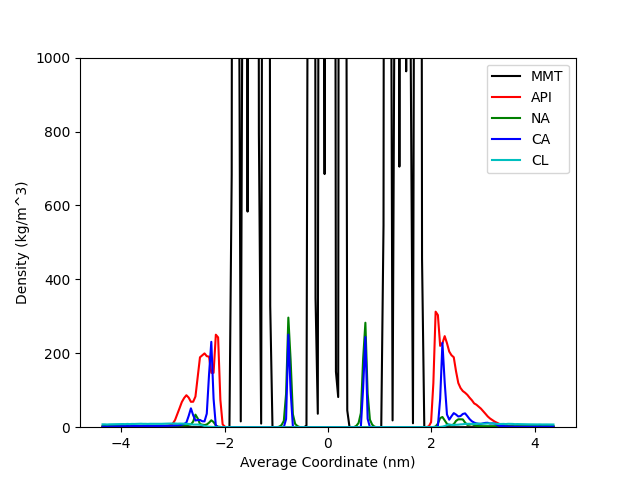
\includegraphics[width=0.8\textwidth]{my_plot.png}
      \caption{An example plot, showing linear density profile for apigenin (API) - clay (MMT) system containing Na$^{+}$, Ca$^{2+}$ and \ce{Cl-} ions. Water is present but not shown.}
      \label{fig:plot}
    \end{minipage}
\end{figure}


\begin{figure}[h!]
    \begin{minipage}{\linewidth}
      \centering
      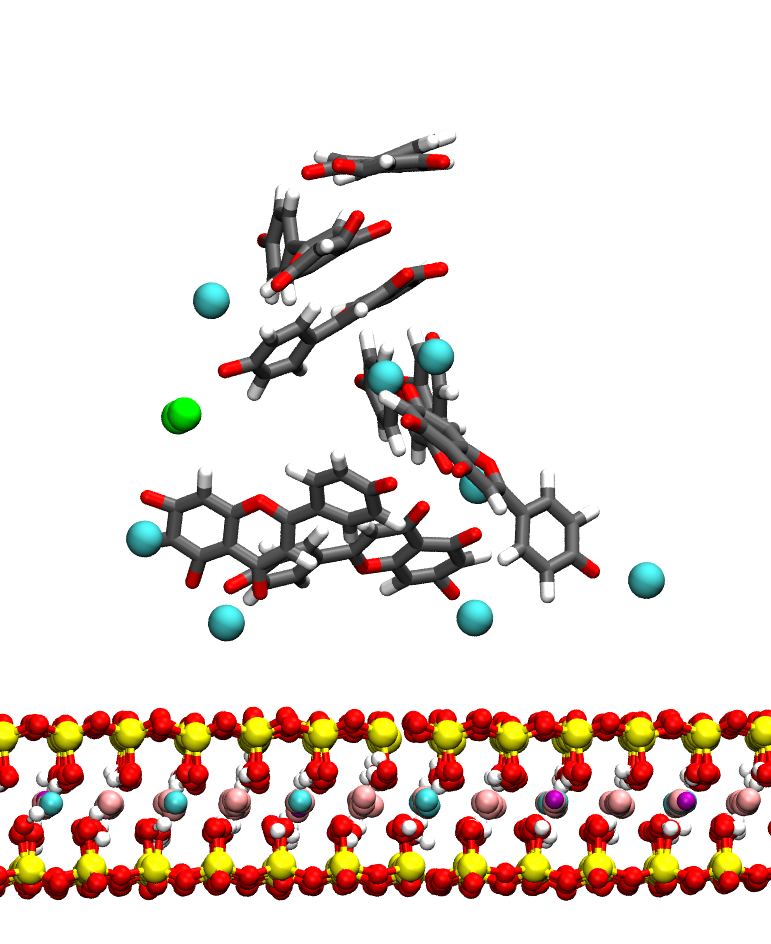
\includegraphics[width=0.5\textwidth]{my_rendering.png}
      \caption{This is an example rendering, showing an interaction between apigenin molecules and clay surface in the presence of ions.  Colours are as follows: C - grey, H - white, O - red, Si - yellow, Al - cyan, Mg - pink, Fe - purple, \ce{Ca^{2+}} - large cyan spheres, \ce{Cl-} - green spheres. Water is not shown for clarity.}
      \label{fig:render}
  \end{minipage}
\end{figure}

You may want to include a table (Table \ref{tab:results}) summarising your results. Note that typically figures have captions below and tables above.



\begin{table}[h!]
    \centering
    \caption{This is an example table, showing Parameter 1 and Parameter 2 for Set I and Set II.}
    \label{tab:results}
    \begin{tabular}{c | c c}
         Name &  Parameter 1 (kg m$^{-3}$) &  Parameter 2 (m$^{3}$) \\
         \hline
         Set I & 11 $\pm$ 3  & 0.34  \\
         Set II & 33 $\pm$ 4  & 0.56 \\
    \end{tabular}
\end{table}



To download a PDF file for submission, make sure you have compiled your most recent version, then click 'Menu' on the top left and then select 'PDF'.

%%%%%%% Conclusions %%%%%%%

\section*{Conclusions}
\textbf{\color{blue}{Approx. 100 words including tables and captions.\\
Outline the key conclusions from your study.}}


\textbf{\color{blue}{Overall, your report should be about 1500 words and include a figure of the system, an analysis plot and possibly a table. }}

% go to the new page
\newpage 

% References section 

\printbibliography %Prints bibliography

\end{document}
